\subsection{Work sharing}

\textbf{Work-sharing constructs divide the execution of a region of code among the team members who encounter it}. A work-sharing construct must be enclosed in a parallel region for the directive to be executed in parallel. Note that the \textbf{constructs do not start new threads}. Also, there is \textbf{\underline{no} implicit barrier at the \emph{entry}} of a work-sharing construct, but \textbf{\underline{there is} an implicit barrier at the \emph{exit}} of a work-sharing construct.

\longline

\subsubsection{For}

The for directive \textbf{shares iterations of a loop across the team} (data parallelism).
\begin{figure}[!htp]
    \centering
    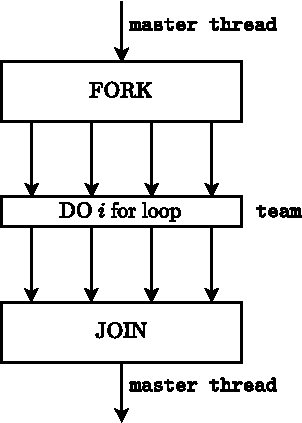
\includegraphics[width=.3\textwidth]{img/openmp-for-1.pdf}
    \caption{OpenMP for loop.}
\end{figure}

\noindent
\begin{openmpbox}[: \texttt{pragma omp for}]
\begin{lstlisting}[language=C++]
#pragma omp parallel
{
    #pragma omp for
    /* for loop */
}\end{lstlisting}
\end{openmpbox}

\noindent
The for directive parallelize execution of iterations. The number of iteration cannot be internally modified. Some common clauses are:
\begin{itemize}
    \item \texttt{\emph{schedule}} that describes \textbf{how iterations of the loop are distributed among the threads in the team}. The schedule type can be either \texttt{dynamic}, \texttt{guided}, \texttt{runtime}, or \texttt{static}.
    \begin{itemize}
        \item \texttt{\emph{static}}. Loop \textbf{iterations are divided into blocks of size \texttt{chunk}} and then statically allocated to threads. If \texttt{chunk} is \textbf{\underline{not} specified}, the \textbf{iterations are divided evenly} (if possible) \textbf{among the threads}.
        \newpage
        \begin{figure}[!htp]
            \centering
            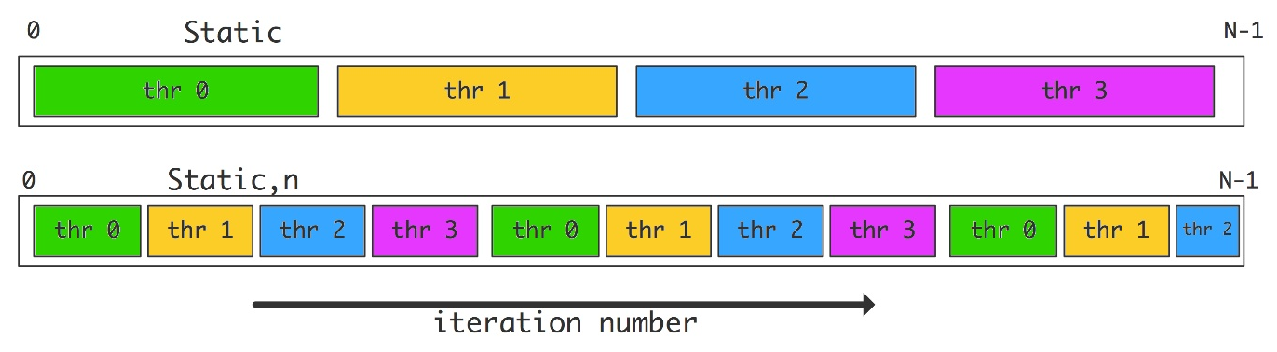
\includegraphics[width=\textwidth]{img/openmp-for-2.pdf}
            \caption{\texttt{static} schedule.}
        \end{figure}

        \item \texttt{\emph{dynamic}}. Loop \textbf{iterations are divided into blocks of size \texttt{chunk}} and \textbf{distributed among the threads \emph{at runtime}}; when a thread completes one chunk, it is \textbf{dynamically allocated another}. The default chunk size is 1. In fact, we can see in the image that the order is not always the same.
        \begin{figure}[!htp]
            \centering
            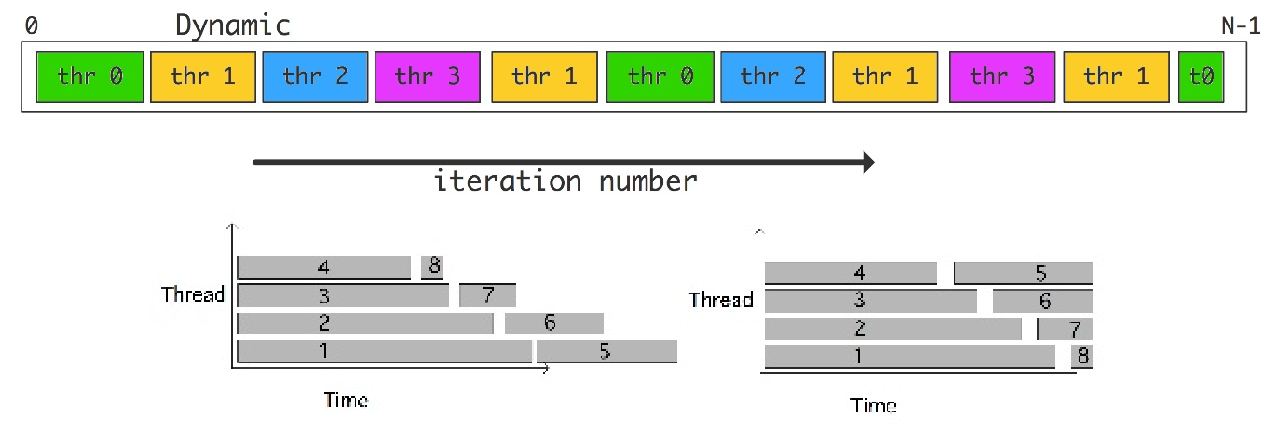
\includegraphics[width=\textwidth]{img/openmp-for-3.pdf}
            \caption{\texttt{dynamic} schedule.}
        \end{figure}
        
        \item \texttt{\emph{runtime}}. Depends on environment variable \texttt{OMP\_SCHEDULE}.

        \item \texttt{\emph{guided}}. Static, gradually decreases the chunk size (\texttt{chunk} specifies the smallest one).
        \begin{figure}[!htp]
            \centering
            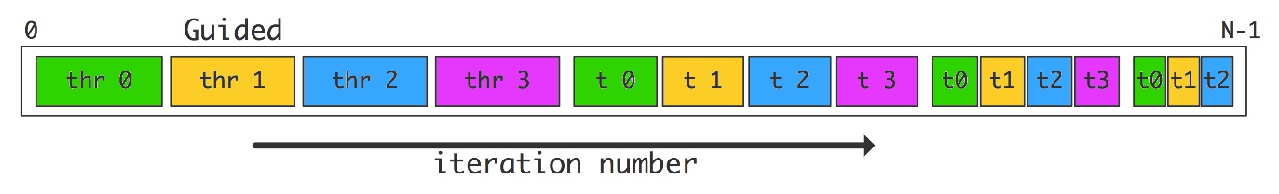
\includegraphics[width=\textwidth]{img/openmp-for-4.pdf}
            \caption{\texttt{guided} schedule.}
        \end{figure}
    \end{itemize}
    \newpage
    \begin{examplebox}[: \texttt{schedule} types]
\begin{lstlisting}[language=C++]
#include <stdio.h>
#include <omp.h>

#define NUM_THREADS 4
#define STATIC_CHUNK 5
#define DYNAMIC_CHUNK 5
#define NUM_LOOPS 20
#define SLEEP_EVERY_N 3

int main( )
{
    int nStatic1[NUM_LOOPS],
        nStaticN[NUM_LOOPS];
    int nDynamic1[NUM_LOOPS],
        nDynamicN[NUM_LOOPS];
    int nGuided[NUM_LOOPS];

    omp_set_num_threads(NUM_THREADS);

    #pragma omp parallel
    {
        #pragma omp for schedule(static, 1)
        for (int i = 0 ; i < NUM_LOOPS ; ++i)
        {
            if ((i % SLEEP_EVERY_N) == 0)
                Sleep(0);
            nStatic1[i] = omp_get_thread_num( );
        }

        #pragma omp for schedule(static, STATIC_CHUNK)
        for (int i = 0 ; i < NUM_LOOPS ; ++i)
        {
            if ((i % SLEEP_EVERY_N) == 0)
                Sleep(0);
            nStaticN[i] = omp_get_thread_num( );
        }

        #pragma omp for schedule(dynamic, 1)
        for (int i = 0 ; i < NUM_LOOPS ; ++i)
        {
            if ((i % SLEEP_EVERY_N) == 0)
                Sleep(0);
            nDynamic1[i] = omp_get_thread_num( );
        }

        #pragma omp for schedule(dynamic, DYNAMIC_CHUNK)
        for (int i = 0 ; i < NUM_LOOPS ; ++i)
        {
            if ((i % SLEEP_EVERY_N) == 0)
                Sleep(0);
            nDynamicN[i] = omp_get_thread_num( );
        }

        #pragma omp for schedule(guided)
        for (int i = 0 ; i < NUM_LOOPS ; ++i)
        {
            if ((i % SLEEP_EVERY_N) == 0)
                Sleep(0);
            nGuided[i] = omp_get_thread_num( );
        }
    }

    printf_s("------------------------------------------------\n");
    printf_s("| static | static | dynamic | dynamic | guided |\n");
    printf_s("|    1   |    %d   |    1    |    %d    |        |\n",
                STATIC_CHUNK, DYNAMIC_CHUNK);
    printf_s("------------------------------------------------\n");

    for (int i=0; i<NUM_LOOPS; ++i)
    {
        printf_s("|    %d   |    %d   |    %d    |    %d    |"
                    "    %d   |\n",
                    nStatic1[i], nStaticN[i],
                    nDynamic1[i], nDynamicN[i], nGuided[i]);
    }

    printf_s("------------------------------------------------\n");
}\end{lstlisting}
    The result will be:
\begin{lstlisting}
------------------------------------------------
| static | static | dynamic | dynamic | guided |
|    1   |    5   |    1    |    5    |        |
------------------------------------------------
|    0   |    0   |    0    |    2    |    1   |
|    1   |    0   |    3    |    2    |    1   |
|    2   |    0   |    3    |    2    |    1   |
|    3   |    0   |    3    |    2    |    1   |
|    0   |    0   |    2    |    2    |    1   |
|    1   |    1   |    2    |    3    |    3   |
|    2   |    1   |    2    |    3    |    3   |
|    3   |    1   |    0    |    3    |    3   |
|    0   |    1   |    0    |    3    |    3   |
|    1   |    1   |    0    |    3    |    2   |
|    2   |    2   |    1    |    0    |    2   |
|    3   |    2   |    1    |    0    |    2   |
|    0   |    2   |    1    |    0    |    3   |
|    1   |    2   |    2    |    0    |    3   |
|    2   |    2   |    2    |    0    |    0   |
|    3   |    3   |    2    |    1    |    0   |
|    0   |    3   |    3    |    1    |    1   |
|    1   |    3   |    3    |    1    |    1   |
|    2   |    3   |    3    |    1    |    1   |
|    3   |    3   |    0    |    1    |    3   |
------------------------------------------------\end{lstlisting}
    \end{examplebox}

    \newpage
    \item \texttt{\emph{nowait}} to \textbf{avoid synchronization at the end of the parallel loop}. It overrides the barrier implicit in a directive.
    \begin{lstlisting}[language=C++]
#pragma omp for nowait\end{lstlisting}
    \begin{examplebox}[: \texttt{nowait} clause]
\begin{lstlisting}[language=C++]
#include <stdio.h>

#define SIZE 5

void test(int *a, int *b, int *c, int size)
{
    int i;
    #pragma omp parallel
    {
        #pragma omp for nowait
        for (i = 0; i < size; i++)
            b[i] = a[i] * a[i];

        #pragma omp for nowait
        for (i = 0; i < size; i++)
            c[i] = a[i]/2;
    }
}

int main( )
{
    int a[SIZE], b[SIZE], c[SIZE];
    int i;

    for (i=0; i<SIZE; i++)
        a[i] = i;

    test(a,b,c, SIZE);

    for (i=0; i<SIZE; i++)
        printf_s("%d, %d, %d\n", a[i], b[i], c[i]);
}\end{lstlisting}
    The output will be:
\begin{lstlisting}
0, 0, 0
1, 1, 0
2, 4, 1
3, 9, 1
4, 16, 2\end{lstlisting}
    \end{examplebox}
\end{itemize}

\newpage

\subsubsection{Sections}

\subsubsection{Single/Master}